\chapter{Method}

\section{Discriminating Variables}

\section{Analysis Overview}
A data-driven method is used to predict the background yield in the
signal regions, as well as the uncertainties on those
predictions. First, jet mass templates are created from control region jets.
Randomized jet masses, known as dressed masses, are generated from
these templates for each jet in the kinematic sample. Summing the
dressed masses for each of the up to four leading jets in an event gives the
dressed $M_{J}^{\Sigma}$ for that event. The dressed $M_{J}^{\Sigma}$
distribution for each signal region is
used to estimate the expected background contribution to that region.

\subsection{Jet mass templates}
Separate templates are created for b-matched and non-b-matched jets. A
b-matched jet is defined as a large-R jet within $\Delta R = 1.0$ of
a b-tagged small-R jet. For the b-matched templates, only events with
$|\Delta \eta_{1,2}| > 1.4$ are included in the templates.

Templates are binned in $p_T$ and $|\eta|$. The $p_T$ bins are
approximately logarithmic, while the $|\eta|$ bin boundaries are at
$0.0$, $0.5$, $1.0$, and $1.5$. 

The template binning and number of jets contributing to each bin are
shown in figure \ref{fig:template_stats}.

\begin{figure}[h]
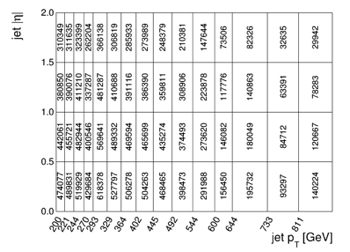
\includegraphics[width=0.5\textwidth]{template_stats_bU}
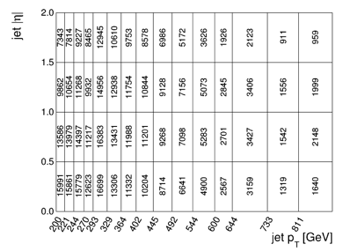
\includegraphics[width=0.5\textwidth]{template_stats_bM}
\caption{Number of jets contributing to each template bin for the
  non-b-matched (left) and b-matched (right) templates.}
\label{fig:template_stats}
\end{figure}

Each template is a one-dimensional histogram of $\log\left(m/p_{T}\right)$,
with $50$ bins. Jets with $\log\left(m/p_{T}\right)< -7$ are excluded
from the templates.

\subsection{Dressed Mass}
For each jet in the kinematic region, a dressed mass is generated by sampling from
the template corresponding to its $p_T$, $|\eta|$ and b-match bin. To
generate a dressed mass, the empirical cumulative distribution fucntion (ECDF)
is calculated for the template. A uniform random number, $y$, in the
range $[0,1)$ is then
generated. The inverse of the ECDF, $\Phi^{-1}(y)$, gives a randomized
$\log\left(m/p_T\right)$ bin. A second uniform random number, $x$, is sampled from the range
$[x_1$,$x_2)$, where $x_1,x_2$ are the edges of the selected bin. The
dressed mass is then computed as $m_{dressed} = p_{T}e^x$.

To obtain a dressed $M_{J}^{\Sigma}$ for an event, one dressed mass is
generated for each jet, and the dressed masses are summed. For
events with more than four jets, only the first four leading jets are
included in the sum.


\section{Event Selection}
\section{Control, Validation, and Signal Regions}
\section{Data-Driven Background Uncertainty Estimation Method}
\subsection{Uncertainty Determination Regions}
\subsection{Dressed Mass Response}

Dressed mass response plots are created by plotting the average
dressed and kinematic jet mass in each $p_T$ bin. The dressed mass
response for the control region is shown in figure
\ref{fig:response_3jCR}. Good agreement between average dressed and
kinematic masses is observed. 

\begin{figure}[h]
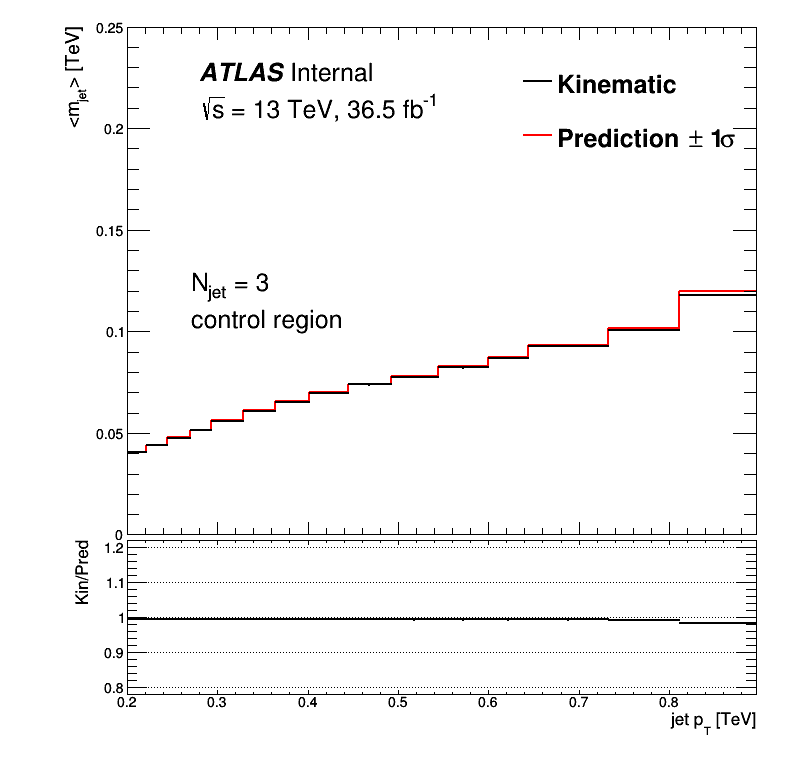
\includegraphics[width=0.6\textwidth]{plot_mass_response_3jCR}
\centering
\caption{Average dressed and kinematic jet masses for each $p_T$ bin
  in the control region}
\label{fig:response_3jCR}

\end{figure}

\subsection{Uncertainty Determination}
\section{Background Estimation Method Applied to MC}




\subsubsection{Dressed $M_{J}^{\Sigma}$ distributions}
To obtain the nominal dressed $M_{J}^{\Sigma}$ distribution,
$n_{toys}$ histograms of $M_{J}^{\Sigma}$ are created, where each
histogram is generated by dressing all events in the sample once. For
each $M_{J}^{\Sigma}$ bin, the average bin content over all histograms is taken
as the nominal value, and the standard deviation of bin contents is
taken as the statistical uncertainty.

The $M_{J}^{\Sigma}$ histograms are binned in the following
manner. There are ten equal-width bins covering the range $0~TeV \leq M_{J}^{\Sigma} <
0.5~TeV$. The next three bins cover the ranges $0.5~TeV \leq M_{J}^{\Sigma} <
0.6~TeV$, $0.6~TeV \leq M_{J}^{\Sigma} <
0.8~TeV$, and $0.8~TeV \leq M_{J}^{\Sigma} <
1.0~TeV$. The final bin is $M_{J}^{\Sigma} \geq
1.0~TeV$
\subsubsection{Normalization}
The dressed $M_{J}^{\Sigma}$ distributions are scaled such that the
dressed yield in the range  $0.2~TeV < M_{J}^{\Sigma} <
0.4~TeV$ is equal to the kinematic yield in the same range. Separate
scale factors are derived for each of the validation and signal regions.

\subsection{Systematic uncertainty}
Systematic uncertainties are derived from the dressed mass response in
the UDRs.

\subsubsection{Binning of systematics}
Systematic uncertainties are binned in $p_{T}$ and $|\eta|$. The lowest
$p_{T}$ bin is for jets with $p_{T} < 402~GeV$. The second bin is for
jets with $402~GeV \leq p_T
< 544~GeV$, and the highest bin is for jets with $p_T \geq 544~GeV$.

\subsubsection{Deriving uncertainty}
For jets with $p_{T} \geq 402~GeV$, uncertainties are derived only
from UDR1.

For jets with $p_{T} < 402~GeV$, uncertainties are derived from both
UDR1 and UDR2, and the maximum uncertainty is used.

For each $p_T$ bin in the UDR dressed mass response, a fractional
error is calculated as
$e_i=\left(<m_{kin}>-<m_{dressed}>\right)/<m_{dressed}>$.

For the lowest and highest $p_T$ systematic bins, the root-mean-square
of fractional errors is taken as the systematic error. For the
intermediate systematic bin, the maximum fractional error is taken

\subsubsection{Propagation of uncertainty}
Two separate systematic uncertainties are derived. The first
uncertainty accounts for the discrepancy between dressed and kinematic
masses for jets with $p_T \geq 402~GeV$, and the second accounts for the
discrepancy for jets with $p_T < 402~GeV$.

To propagate the low-$p_T$ systematic, two shifted $M_{J}^{\Sigma}$
values are calculated for each dressed $M_{J}^{\Sigma}$. The first
shifted value is obtained by increasing the dressed mass of every
low-$p_T$ jet by its corresponding fractional uncertainty. This yields
$n_{toys}$ histograms of shifted $M_{J}^{\Sigma}$. The average value
of each bin content over all toys is taken to obtain the
systematically-shifted $M_{J}^{\Sigma}$ distribution. 

The second
shifted distribution is obtained by decreasing the dressed mass of every
low-$p_T$ jet by its corresponding fractional uncertainty, and
averaging over all the toys to obtain a downwards-shifted distribution
of $M_{J}^{\Sigma}$. 

The same procedure is used to propagate the high-$p_T$ systematic, but
the high-$p_T$ jets are shifted instead of the low-$p_T$ jets.

\subsection{Determining predicted $M_{J}^{\Sigma}$ and uncertainties}
To determine the nominal predicted background yield, one thousand toys
are generated, where a toy consists of a dressed $M_{J}^{\Sigma}$ value for
each event in the kinematic sample. For each toy, the number of events
with dressed $M_{J}^{\Sigma}$ greater than the signal region
$M_{J}^{\Sigma}$ cut are counted, giving a distribution of one
thousand dressed background yields. The central value of this distribution is
multiplied by the scale factor to obtain the nominal background
prediction. The standard deviation of this distribution is multiplied
by the scale factor to obtain the statistical uncertainty on the
background prediction.

Systematically-shifted background yield predictions are determined by repeating
the above procedure for the systematically-shifted dressed
$M_{J}^{\Sigma}$ values. The systematic uncertainties are taken as the
difference between the nominal and systematically-shifted background
yield predictions. Scale factors are only derived from the nominal
$M_{J}^{\Sigma}$ distributions and applied to both the nominal and
systematically-shifted predictions.

The two systematic uncertainties are symmetrized by taking the maximum
of the downward-shifted and upward-shifted uncertainties.
\section{Signal Modeling}
\section{Systematic Uncertainties}
\subsection{Background Systematics}
\subsection{Signal Systematics}
\section{Signal Contamination}
